\documentclass[
    % MENDT6 item 2
	% -- opções da classe memoir --
	12pt,				% tamanho da fonte
	openright,			% capítulos começam em pág ímpar (insere página vazia caso preciso)
	oneside,			% [oneside or twoside]para impressão em recto e verso. Oposto a oneside (acordo MENDT6 é opcional 1 ou 2 lados, prefenrencialmente 2 lados)
	a4paper,			% tamanho do papel. 
	% -- opções da classe abntex2 --
	chapter=TITLE,		% títulos de capítulos convertidos em letras maiúsculas
	%section=TITLE,		% títulos de seções convertidos em letras maiúsculas
	%subsection=TITLE,	% títulos de subseções convertidos em letras maiúsculas
	%subsubsection=TITLE,% títulos de subsubseções convertidos em letras maiúsculas
	% -- opções do pacote babel --
	english,			% idioma adicional para hifenização
	french,				% idioma adicional para hifenização
	%spanish,			% idioma adicional para hifenização
	brazil				% o último idioma é o principal do documento
	]{abntex2}

% ---
% Pacotes básicos 
% ---
\usepackage{lmodern}			% Usa a fonte Latin Modern			
\usepackage[T1]{fontenc}		% Selecao de codigos de fonte.
\usepackage[utf8]{inputenc}		% Codificacao do documento (conversão automática dos acentos)
\usepackage{indentfirst}		% Indenta o primeiro parágrafo de cada seção.
\usepackage{color}				% Controle das cores
\usepackage{graphicx}			% Inclusão de gráficos
\usepackage{microtype} 			% para melhorias de justificação
% ---
	
% ---
% Pacotes adicionais, usados apenas no âmbito do Modelo Canônico do abnteX2
% ---
\usepackage{amsfonts}
\usepackage{amssymb} 
\usepackage{amsthm}
\usepackage{amsmath}
\usepackage{bm}
\usepackage{comment}
\usepackage{enumerate}

%\usepackage{lipsum}				% para geração de dummy text
\usepackage{tikz}
\usetikzlibrary{positioning}
\usepackage{xcolor}
\usepackage{array}     % Elementos extras para formatação de tabelas

% ---

% ---
% Pacotes de citações
% ---
\usepackage[brazilian,hyperpageref]{backref}	 % Paginas com as citações na bibl
% MENDT6 - podem ser númerica ou autor/data
\usepackage[num]{abntex2cite}	% Citações padrão ABNT 
%\usepackage[alf]{abntex2cite}	% Citações padrão ABNT 

% --- 
% CONFIGURAÇÕES DE PACOTES
% --- 
% Configurações do pacote backref
% Usado sem a opção hyperpageref de backref
\renewcommand{\backrefpagesname}{Citado na(s) página(s):~}
% Texto padrão antes do número das páginas
\renewcommand{\backref}{}
% Define os textos da citação
\renewcommand*{\backrefalt}[4]{
	\ifcase #1 %
		Nenhuma citação no texto.%
	\or
		Citado na página #2.%
	\else
		Citado #1 vezes nas páginas #2.%
	\fi}%

% ------------------------------------------------------------------------
% Informações de dados para CAPA e FOLHA DE ROSTO
% Preenchimento obrigatório

% ---
% Informações de dados para CAPA e FOLHA DE ROSTO
% ---
\titulo{Corretude de programas concorrentes baseados em troca de mensagem}
\autor{Saulo Andrade Almeida}
\local{Rio de Janeiro, Brasil}
\data{2023, v-1.0.0}
\orientador[D.Sc.]{Silvana Rossetto}
\instituicao{%
    Universidade Federal do Rio de Janeiro -- UFRJ
    \par
    Instituto de Computação
    \par
    Instituto Tércio Pacitti de Aplicações e Pesquisas Computacionais
    \par
    Programa de Pós-Graduação em Informática}
\tipotrabalho{Dissertação (Mestrado)}
% O preambulo deve conter o tipo do trabalho, o objetivo, 
% o nome da instituição e a área de concentração 
\preambulo{Qualificação de Mestrado a ser submetida à banca de Corpo Docente selecionada pelo Programa de Pós-Graduação em Informática, Instituto Tércio Pacitti de Aplicações e Pesquisas Computacionais, Instituto de Computação da Universidade Federal do Rio de Janeiro. Área de Concentração Informática.}
% ---
% ------------------------------------------------------------------------

% ------------------------------------------------------------------------
% informações do PDF
\makeatletter
% informações do PDF

\hypersetup{
     	%pagebackref=true,
		pdftitle={\@title}, 
		pdfauthor={\@author},
    	pdfsubject={\imprimirpreambulo},
	    pdfcreator={LaTeX with abnTeX2},
		pdfkeywords={programação paralela}{concorrência}{verificação de erros}{SLR}{revisão de literatura sistemática}, 
		colorlinks=true,       		% false: boxed links; true: colored links
    	linkcolor=blue,          	% color of internal links
    	citecolor=blue,        		% color of links to bibliography
    	filecolor=magenta,      		% color of file links
		urlcolor=blue,
		bookmarksdepth=4
}
\makeatother
% ------------------------------------------------------------------------
 
% ---
% Posiciona figuras e tabelas no topo da página quando adicionadas sozinhas
% em um página em branco. Ver https://github.com/abntex/abntex2/issues/170
\makeatletter
\setlength{\@fptop}{5pt} % Set distance from top of page to first float
\makeatother
% ---

% ---
% Possibilita criação de Quadros e Lista de quadros.
% Ver https://github.com/abntex/abntex2/issues/176
%
\newcommand{\quadroname}{Quadro}
\newcommand{\listofquadrosname}{Lista de quadros}

\newfloat[chapter]{quadro}{loq}{\quadroname}
\newlistof{listofquadros}{loq}{\listofquadrosname}
\newlistentry{quadro}{loq}{0}

% configurações para atender às regras da ABNT
\setfloatadjustment{quadro}{\centering}
\counterwithout{quadro}{chapter}
\renewcommand{\cftquadroname}{\quadroname\space} 
\renewcommand*{\cftquadroaftersnum}{\hfill--\hfill}
\pdfstringdefDisableCommands{\let\uppercase\relax}

\setfloatlocations{quadro}{hbtp} 
% Ver https://github.com/abntex/abntex2/issues/176
% ---

% --- 
% Espaçamentos entre linhas e parágrafos 
% --- 

% O tamanho do parágrafo é dado por:
\setlength{\parindent}{1.3cm}

% Controle do espaçamento entre um parágrafo e outro:
\setlength{\parskip}{0.2cm}  % tente também \onelineskip

% ---
% compila o indice
% ---
\makeindex
% ---

% ------------------------------------------------------------------------
% Definições pessoais extras para serem incluídas no cabeçalho do
% documento LaTex.
%=====================================================================
%% Declaration to use comments into text, in a revision fase
%booleandeclaration
\newboolean{REVISION}
% Turn ON comments:true / Turn OFF comments:false
\setboolean{REVISION}{true} % <---------

\definecolor{violet}{rgb}{0.56,0.0,1.0}
\definecolor{brightmaroon}{rgb}{0.76, 0.13, 0.28}
\definecolor{amber}{rgb}{1.0, 0.75, 0.0}

\ifthenelse{\boolean{REVISION}}
{
    \newcommand{\vilc}   [1]{\textcolor{blue}   {[#1 -- VILC]}}
    \newcommand{\sadoc}  [1]{\textcolor{red}    {[#1 -- SADOC]}}
    \newcommand{\icc}    [1]{\textcolor{violet} {[#1 -- CUNHA]}}
    \newcommand{\cabral} [1]{\textcolor{cyan}   {[#1 -- CABRAL]}}
    \newcommand{\michael}[1]{\textcolor{magenta}{[#1 -- MG]}}
%    \newcommand{\fdp}    [1]{\textcolor{black}   {#1}}
%%%%
    \newcommand{\edvilc} [1]{\textcolor{blue}        {#1 -- VILC}}
    \newcommand{\ic}     [1]{\textcolor{violet}      {#1 -- CUNHA}}
    \newcommand{\fdp}    [1]{\textcolor{black}{#1}}
    \newcommand{\RE}     [1]{\textcolor{black}       {#1}}
}{
    \newcommand{\vilc}   [1]{}
    \newcommand{\sadoc}  [1]{}
    \newcommand{\icc}    [1]{}
    \newcommand{\cabral} [1]{}
    \newcommand{\michael}[1]{}
%%%
    \newcommand{\edvilc} [1]{#1}
    \newcommand{\ic}     [1]{#1}
    \newcommand{\fdp}    [1]{#1}
    \newcommand{\RE}     [1]{#1}
} 


%=====================================================================
%% Definition of theorems
\theoremstyle{plain}
%\newtheorem{thm}{Teorema}[section]
\newtheorem{thm}{Theorem}[section]
\newtheorem{lemma}{Lemma}[section]
%\newtheorem{prop}{Proposição}[section]
\newtheorem{prop}{Proposition}[section]
\newtheorem{conjc}{Conjectura}[section]
%\newtheorem{sublem}[lem]{Sub-lemma}
%\newtheorem{def}{Definition}[section]
\newtheorem{cor}{Corollary}[section]
%\newtheorem{prob}{Problem}[section]
%\newtheorem{prpd}{Propriedade}[section]

\newtheorem{theorem}{Theorem}[section]
\newtheorem{corollary}{Corollary}[section]
\newtheorem{definition}{Definition}[section]
\newtheorem{problem}{Problem}[section]
%\newtheorem{conj}[lem]{Conjectura}\renewcommand{\theconj}{}
%\theoremstyle{definition}
%\newtheorem{defi}[thm]{Defini\c c\~ ao}
%\newtheorem{cond}[lem]{Condi\c c\~ ao}
%\theoremstyle{example}
%\newtheorem{exemp}[thm]{Exemplo}
%\newtheorem{rem}[lem]{Remark}
%\newtheorem{alem}{Lema}[section]

%=====================================================================
%% Definitions to TIKZ PACKAGE
\begin{comment}

\usetikzlibrary{positioning}

\definecolor{lavander}{cmyk}{0,0.48,0,0}
\definecolor{violet}{cmyk}{0.79,0.88,0,0}
\definecolor{burntorange}{cmyk}{0,0.52,1,0}

\tikzstyle{state}=[draw,circle,blue, text=violet, inner sep=0pt,minimum width=15pt]  
\tikzstyle{statewhite}=[draw,circle,white, text=violet, inner sep=0pt,minimum width=15pt]  

\end{comment}

%=====================================================================
%% Minimal and maximal declaration in math mode
\DeclareMathOperator*{\argmin}{arg\,min}
\DeclareMathOperator*{\argmax}{arg\,max}


%=====================================================================
%% Shotcut to special characters and symbous
\newcommand{\ind}[1]{1\hspace{-0.125cm}1\{#1\}}
\newcommand{\CR}{ {\mbox{\em CR}} }

\newcommand{\SA}{ {\cal A} }
\newcommand{\SB}{ {\cal B} }
\newcommand{\SC}{ {\cal C} }
\newcommand{\SD}{ {\cal D} }
\newcommand{\SE}{ {\cal E} }
\newcommand{\SF}{ {\cal F} }
\newcommand{\SG}{ {\cal G} }
\newcommand{\SH}{ {\cal H} }
\newcommand{\SI}{ {\cal I} }
\newcommand{\SJ}{ {\cal J} }
\newcommand{\SK}{ {\cal K} }
\newcommand{\SL}{ {\cal L} }
\newcommand{\SM}{ {\cal M} }
\newcommand{\SN}{ {\cal N} }
\newcommand{\SO}{ {\cal O} }
\newcommand{\SP}{ {\cal P} }
\newcommand{\SQ}{ {\cal Q} }
\newcommand{\SR}{ {\cal R} }
\newcommand{\sS}{ {\cal S} }
\newcommand{\ST}{ {\cal T} }
\newcommand{\SU}{ {\cal U} }
\newcommand{\SV}{ {\cal V} }
\newcommand{\SW}{ {\cal W} }
\newcommand{\SX}{ {\cal X} }
\newcommand{\SY}{ {\cal Y} }
\newcommand{\SZ}{ {\cal Z} }
 

\newcommand{\mb}[1]  { {\mbox{\rm #1}} }
\newcommand{\ee}     { {\mbox{e     }} }
\newcommand{\diag}   { {\mbox{diag  }} }

\newcommand{\bGamma} { {\mbox{\boldmath $\Gamma$     }} }
\newcommand{\bLambda}{ {\mbox{\boldmath $\Lambda$    }} }
\newcommand{\bOmega} { {\mbox{\boldmath $\Omega$     }} }
\newcommand{\bUpsilon}{{\mbox{\boldmath $\Upsilon$   }} }
\newcommand{\bPi}    { {\mbox{\boldmath $\Pi$        }} }
\newcommand{\bPsi}   { {\mbox{\boldmath $\Psi$       }} }
\newcommand{\bpi}    { {\mbox{\boldmath $\pi$        }} }
\newcommand{\bphi}   { {\mbox{\boldmath $\phi$       }} }
\newcommand{\bpsi}   { {\mbox{\boldmath $\psi$       }} }
\newcommand{\balpha} { {\mbox{\boldmath $\alpha$     }} }
\newcommand{\bbeta}  { {\mbox{\boldmath $\beta$      }} }
\newcommand{\bmu}    { {\mbox{\boldmath $\mu$        }} }

\newcommand{\bdelta} { {\mbox{\boldmath $\delta$     }} }
\newcommand{\bepsilon}{{\mbox{\boldmath $\epsilon$   }} }
\newcommand{\blambda}{ {\mbox{\boldmath $\lambda$    }} }
\newcommand{\btheta} { {\mbox{\boldmath $\theta$     }} }

\newcommand{\bgamma} { {\mbox{\boldmath $\gamma$     }} }
\newcommand{\bomega} { {\mbox{\boldmath $\omega$     }} }
\newcommand{\btau}   { {\mbox{\boldmath $\tau$       }} }
\newcommand{\bnu}    { {\mbox{\boldmath $\nu$        }} }
\newcommand{\bvarep} { {\mbox{\boldmath $\varepsilon$}} }

\newcommand{\bxi}    { {\mbox{\boldmath $\xi$        }} }
\newcommand{\bzeta}  { {\mbox{\boldmath $\zeta$      }} }
\newcommand{\bvarphi}{ {\mbox{\boldmath $\varphi$    }} }
\newcommand{\bkappa} { {\mbox{\boldmath $\kappa$     }} }
\newcommand{\bsigma} { {\mbox{\boldmath $\sigma$     }} }
\newcommand{\brho}   { {\mbox{\boldmath $\rho$       }} }
\newcommand{\bvarrho}{ {\mbox{\boldmath $\varrho$    }} }
\newcommand{\bPhi}   { {\mbox{\boldmath $\Phi$       }} }


\newcommand{\bA}{ \boldsymbol {A} }
\newcommand{\bB}{ \boldsymbol {B} }
\newcommand{\bC}{ \boldsymbol {C} }
\newcommand{\bD}{ \boldsymbol {D} }
\newcommand{\bE}{ \boldsymbol {E} }
\newcommand{\bF}{ \boldsymbol {F} }
\newcommand{\bG}{ \boldsymbol {G} }
\newcommand{\bH}{ \boldsymbol {H} }
\newcommand{\bI}{ \boldsymbol {I} }
\newcommand{\bJ}{ \boldsymbol {J} }
\newcommand{\bK}{ \boldsymbol {K} }
\newcommand{\bL}{ \boldsymbol {L} }
\newcommand{\bM}{ \boldsymbol {M} }
\newcommand{\bN}{ \boldsymbol {N} }
\newcommand{\bO}{ \boldsymbol {O} }
\newcommand{\bP}{ \boldsymbol {P} }
\newcommand{\bQ}{ \boldsymbol {Q} }
\newcommand{\bR}{ \boldsymbol {R} }
\newcommand{\bS}{ \boldsymbol {S} }
\newcommand{\bT}{ \boldsymbol {T} }
\newcommand{\bU}{ \boldsymbol {U} }
\newcommand{\bV}{ \boldsymbol {V} }
\newcommand{\bW}{ \boldsymbol {W} }
\newcommand{\bX}{ \boldsymbol {X} }
\newcommand{\bY}{ \boldsymbol {Y} }
\newcommand{\bZ}{ \boldsymbol {Z} }

\newcommand{\boo}{\boldsymbol {0} }
\newcommand{\bzr}{\boldsymbol {0} }
\newcommand{\bon}{\boldsymbol {1} }
\newcommand{\ba}{ \boldsymbol {a} }
\newcommand{\bb}{ \boldsymbol {b} }
\newcommand{\bc}{ \boldsymbol {c} }
\newcommand{\bd}{ \boldsymbol {d} }
\newcommand{\be}{ \boldsymbol {e} }
\newcommand{\bff}{\boldsymbol {f} }
\newcommand{\bg}{ \boldsymbol {g} }
\newcommand{\bh}{ \boldsymbol {h} }
\newcommand{\bi}{ \boldsymbol {i} }
\newcommand{\bj}{ \boldsymbol {j} }
\newcommand{\bk}{ \boldsymbol {k} }
\newcommand{\bl}{ \boldsymbol {l} }
\newcommand{\bmm}{ \boldsymbol {m} }
\newcommand{\bn}{ \boldsymbol {n} }
\newcommand{\bo}{ \boldsymbol {o} }
\newcommand{\bp}{ \boldsymbol {p} }
\newcommand{\bq}{ \boldsymbol {q} }
\newcommand{\br}{ \boldsymbol {r} }
\newcommand{\bss}{ \boldsymbol {s} }
\newcommand{\bt}{ \boldsymbol {t} }
\newcommand{\bu}{ \boldsymbol {u} }
\newcommand{\bv}{ \boldsymbol {v} }
\newcommand{\bx}{ \boldsymbol {x} }
\newcommand{\bw}{ \boldsymbol {w} }
\newcommand{\by}{ \boldsymbol {y} }
\newcommand{\bz}{ \boldsymbol {z} }



% ------------------------------------------------------------------------

% ------------------------------------------------------------------------
% Início do documento
\begin{document}

% Seleciona o idioma do documento (conforme pacotes do babel)
%\selectlanguage{english}
\selectlanguage{brazil}

% Retira espaço extra obsoleto entre as frases.
\frenchspacing 

% ------------------------------------------------------------------------
% ------------------------------------------------------------------------
% ------------------------------------------------------------------------
% INÍCIO ELEMENTOS PRE-TEXTUAIS
% ------------------------------------------------------------------------
\pretextual

% ------------------------------------------------------------------------
% Capa
\imprimircapa
% ---

% Folha de rosto
% (o * indica que haverá a ficha bibliográfica)
\imprimirfolhaderosto*
% ---

% Opcional: Ficha catalográfica quando for fazer a
% entrega final do texto

% ---
% Inserir a ficha bibliografica
% ---

% Isto é um exemplo de Ficha Catalográfica, ou ``Dados internacionais de
% catalogação-na-publicação''. Você pode utilizar este modelo como referência. 
% Porém, provavelmente a biblioteca da sua universidade lhe fornecerá um PDF
% com a ficha catalográfica definitiva após a defesa do trabalho. Quando estiver
% com o documento, salve-o como PDF no diretório do seu projeto e substitua todo
% o conteúdo de implementação deste arquivo pelo comando abaixo:
%
% \begin{fichacatalografica}
%     \includepdf{fig_ficha_catalografica.pdf}
% \end{fichacatalografica}

\begin{fichacatalografica}
	\sffamily
	\vspace*{\fill}					% Posição vertical
	\begin{center}					% Minipage Centralizado
	\fbox{\begin{minipage}[c][8cm]{13.5cm}		% Largura
	\small
	\imprimirautor
	%Sobrenome, Nome do autor
	
	\hspace{0.5cm} \imprimirtitulo  / \imprimirautor. --
	\imprimirlocal, \imprimirdata-
	
	\hspace{0.5cm} \thelastpage p. : il. (algumas color.) ; 30 cm.\\
	
	\hspace{0.5cm} \imprimirorientadorRotulo~\imprimirorientador\\
	
	\hspace{0.5cm}
	\parbox[t]{\textwidth}{\imprimirtipotrabalho~--~\imprimirinstituicao,
	\imprimirdata.}\\
	
	\hspace{0.5cm}
		1. Epidemias.
		2. Segurança da Informação.
		3. Atacante estratégico.
		I. Orientador \imprimirorientadorRotulo~\imprimirorientador.
		II. Universidade Federal do Rio de Janeiro.
		III. Programa de Pós-Graduação em Informática.
		IV. \imprimirtitulo			
	\end{minipage}}
	\end{center}
\end{fichacatalografica}
% ---
% ---

% Erratas

% ---
% Inserir errata
% ---
\begin{errata}
%Elemento opcional da \citeonline[4.2.1.2]{NBR14724:2011}. Exemplo:

\vspace{\onelineskip}

%FERRIGNO, C. R. A. \textbf{Tratamento de neoplasias ósseas apendiculares com reimplantação de enxerto ósseo autólogo autoclavado associado ao plasma rico em plaquetas}: estudo crítico na cirurgia de preservação de membro em cães. 2011. 128 f. Tese (Livre-Docência) - Faculdade de Medicina Veterinária e Zootecnia, Universidade de São Paulo, São Paulo, 2011.

\begin{table}[htb]
\center
\footnotesize
\begin{tabular}{|p{1.4cm}|p{1cm}|p{3cm}|p{3cm}|}
  \hline
   \textbf{Folha} & \textbf{Linha}  & \textbf{Onde se lê}  & \textbf{Leia-se}  \\
   \hline
\end{tabular}
\end{table}

\end{errata}
% ---

% ---

% Folha de aprovação
% ---
% Inserir folha de aprovação
% ---


% Isto é um exemplo de Folha de aprovação, elemento obrigatório da NBR
% 14724/2011 (seção 4.2.1.3). Você pode utilizar este modelo até a aprovação
% do trabalho. Após isso, substitua todo o conteúdo deste arquivo por uma
% imagem da página assinada pela banca com o comando abaixo:
%
% \begin{folhadeaprovacao}
% \includepdf{folhadeaprovacao_final.pdf}
% \end{folhadeaprovacao}
%
\begin{folhadeaprovacao}

  \begin{center}
    {\ABNTEXchapterfont\large\imprimirautor}

    \vspace*{\fill}\vspace*{\fill}
    \begin{center}
      \ABNTEXchapterfont\bfseries\Large\imprimirtitulo
    \end{center}
    \vspace*{\fill}
    
    \hspace{.45\textwidth}
    \begin{minipage}{.5\textwidth}
        \imprimirpreambulo
    \end{minipage}%
    \vspace*{\fill}
   \end{center}
        
   Trabalho aprovado. \imprimirlocal, 10 de abril de 2024:

   \assinatura{\textbf{\imprimirorientadorRotulo~\imprimirorientador} \\ Orientador} 
   \assinatura{\textbf{D.Sc. Claudio Miceli de Farias} \\ PPGI-UFRJ}
   \assinatura{\textbf{D.Sc.Edmundo Albuquerque de Souza e Silva} \\ PESC-UFRJ}
   \assinatura{\textbf{D.Sc Alberto Avritzer} \\ ESULABSOLUTIONS}
   %\assinatura{\textbf{Professor} \\ Convidado 4}
      
   \begin{center}
    \vspace*{0.5cm}
    {\large\imprimirlocal}
    \par
    {\large\imprimirdata}
    \vspace*{1cm}
  \end{center}
  
\end{folhadeaprovacao}
% ---

% Dedicatória

% ---
% Dedicatória
% ---
\begin{dedicatoria}
   \vspace*{\fill}
   \centering
   \noindent
   \textit{ Este trabalho é dedicado à minha esposa Munique Falcão Fróes \\
   e minha filha Sofia Fróes Andrade Almeida, \\
   por todo amor, apoio, paciência e compreensão.} \vspace*{\fill}
\end{dedicatoria}
% ---
% ---

% Agradecimentos


% ---
% Agradecimentos
% ---
\begin{agradecimentos}
Os agradecimentos principais são direcionados aos meus pais, Denize Andrade Almeida e Ivan Souza Almeida por todo amor, empenho e valores passados em minha criação. Aos Irmãos Ivan Andrade Almeida e Debora Andrade Almeida, por toda a vivencia e companheirismo. Para minha esposa, amiga e companheira Munique Falcão Fróes, por todo amor, parceria e cumplicidade vividas nas últimas décadas. Para minha filha Sofia Fróes Andrade Almeida, por me ensinar novas dimensões das palavras Amor e Orgulho.

Agradecimentos especiais são direcionados à minha orientadora \imprimirorientador, por sua paciência e por todas as horas de dedicação. Obrigado por sempre acreditar que seria capaz de realizar esse trabalho, mesmo tendo ciência de todas as dificuldades e da pouca disponibilidade de tempo que eu dispunha.

\end{agradecimentos}
% ---

% Epígrafe
% ---
% Epígrafe
% ---
\begin{epigrafe}
    \vspace*{\fill}
	\begin{flushright}
		\textit{``Se é a crise que abre caminho para o progresso, ela deixa de ser crise. \\
		Podemos compará-la à pausa para tomar fôlego, na corrida, ou aos nós do bambu. \\
		As varas do bambu se mantêm firmes devido à formação de nós no curso de seu desenvolvimento; se lhes faltassem nós, não apresentariam sua conhecida resistência. \\
		Quanto mais nós tem o bambu, mais forte ele é.`` \\
		(Mokiti Okada, Alicerce do Paraíso, Vol. 4)}
	\end{flushright}
\end{epigrafe}
% ---

% ------------------------------------------------------------------------
% RESUMOS

% resumo em português
\setlength{\absparsep}{18pt} % ajusta o espaçamento dos parágrafos do resumo
\begin{resumo}
Nos últimos anos a maneira mais eficaz para se realizar otimização no tempo de execução dos processamentos é feita através da paralelização dos processos durante a execução dos programas. O hardware dos mais variados tipos de dispositivos que possuem poder computacional atualmente, como micro-computadores ou dispositivos móveis, habitual mente já possuem arquitetura que permite a realização dos seus processamentos de forma paralela.
Nesse contexto, o desenvolvimento de programas que podem ser executados de forma paralela tem sido cada vez mais necessário e utilizado por uma maior quantidade de desenvolvedores. fórmulas fechadas que  aproximam a probabilidade de infecção e contrastamos os \emph{insights} do modelo com simulações. Simulações suportam qualitativamente as observações do modelo epidêmico e estendem a análise permitindo distribuições gerais.

 \textbf{Palavras-chave}: programação paralela, problemas de concorrência, verificação de erros, SLR, revisão de literatura sistemática.
\end{resumo}

% resumo em inglês
\begin{resumo}[Abstract]
 \begin{otherlanguage*}{english}
   Every day systems are compromised by malicious code and participate in campaigns to attack computer systems.
Thus, users face a dilemma as to which countermeasures to take: harsh (for example, vaccination), mild (for example, restart and rejuvenation) or no countermeasures. To resolve this dilemma, one option is to take advantage of analytical models. In this work, we present a proposal to characterize the steady state of epidemic models in which the attacker is strategic and has a finite attack capacity. For that, the most probable states of the model are analyzed, indicating their properties; closed formulas are presented that approximate the probability of infection and we contrast the \textit{insights} of the model with simulations. Simulations qualitatively support the observations of the epidemic model and extend the analysis by allowing general distributions.

   \vspace{\onelineskip}
 
   \noindent 
   \textbf{Keywords}: latex. epidemic, network contamination, information security.
 \end{otherlanguage*}
\end{resumo}

% ------------------------------------------------------------------------
% LISTAS
% ---
% Preenchidas automaticamente pelo modelo:
% Inserir lista de ilustrações
\pdfbookmark[0]{\listfigurename}{lof}
\listoffigures*
\cleardoublepage
% Inserir lista de quadros
\pdfbookmark[0]{\listofquadrosname}{loq}
\listofquadros*
\cleardoublepage
% Inserir lista de tabelas
\pdfbookmark[0]{\listtablename}{lot}
\listoftables*
\cleardoublepage
% ---
% Preenchido manualmente pelo autor
% Abreviaturas e siglas

% ---
% inserir lista de abreviaturas e siglas
% ---
\begin{siglas}
  \item[DHS] Distributed and Heterogeneous Systems
  \item[abnTeX] ABsurdas Normas para TeX
\end{siglas}
% ---
% Símbolos

% ---
% inserir lista de símbolos
% ---
\begin{simbolos}
  \item[$ \Gamma $] Letra grega Gama
  \item[$ \Lambda $] Lambda
  \item[$ \zeta $] Letra grega minúscula zeta
  \item[$ \in $] Pertence
\end{simbolos}
% ---
% ------------------------------------------------------------------------
%
% SUMÁRIO
% ---
\pdfbookmark[0]{\contentsname}{toc}
\tableofcontents*
\cleardoublepage
% ---
% ------------------------------------------------------------------------
% FIM ELEMENTOS PRE-TEXTUAIS
% ------------------------------------------------------------------------
% ------------------------------------------------------------------------
% ------------------------------------------------------------------------



% ------------------------------------------------------------------------
% ------------------------------------------------------------------------
% ----------------------------------------------------------
% ELEMENTOS TEXTUAIS
% ----------------------------------------------------------
\textual
% ---------------------------------------------------------
% ----------------------------------------------------------
% PARTE
% Não é prevista na MENDT6, porém pode ser necessário 
% minha dica é não use.
% ----------------------------------------------------------
% \part{Imunidade Coletiva diante de atacantes estratégicos}
% ----------------------------------------------------------
% Introdução

\chapter{INTRODUÇÃO}

A programação concorrente não é mais utilizada apenas para resolver problemas relacionados com a computação de alta performance. Os microprocessadores que permitem executar programas concorrentes estão disponíveis em quase todos os dispositivos. Essa nova realidade foi vislumbrada em \cite{sutter_software_2005}, e apresentada como a Revolução do Software Concorrente.

Um programa é dito concorrente quando é construído com o propósito de resolver um ou mais problemas, utilizando mais de uma linha de execução simultânea. 

Atualmente a programação concorrente é utilizada para resolver problemas corriqueiros do desenvolvimento de softwares, como por exemplo: Desacoplar interface de uma aplicação das operações mais demoradas, como as de IO ou de processamentos do back-end; Possibilitar que programas que são executados em um único nó, possa utilizar recursos de arquiteturas multi-core; Na implementação do paradigma de comunicação utilizado pela programação Web, tanto no lado do cliente quanto no lado servidor; Para auxiliar aplicações mobiles nas suas interações com serviços e dados remotos; Em soluções que se apoiam no paradigma  \textit{peer-to-peer}, seja na implementação de serviços ou na coordenação do processamento em múltiplos nós. 

Apesar da programação concorrente ser objeto de estudo desde a década de sessenta \cite{1965Dijkstra}, é possível perceber que nos últimos anos a sua utilização tem sido cada vez mais incentivada, e isso pode ser notado ao avaliar a evolução das novas arquiteturas de hardware com o enfoque na disponibilização de recursos de concorrência ou com a evolução e criação de novas de linguagens de programação com o proposito de viabilizar ou facilitar a utilização desse tipo de programação.

\section{Motivação}

Para garantir o funcionamento correto de um programa que utiliza múltiplos fluxos de processamento, muitas vezes é necessário realizar algum tipo de comunicação ou sincronização das tarefas entre esses fluxos de processamento. Essa necessidade cria novos desafios de designs e de verificação da confiabilidade do programa.

Durante a criação de um programa, apenas a mudança do paradigma de programação sequencial para o de programação concorrente, já cria uma complexidade na forma de pensar o algoritmo, o que normalmente impacta na confiabilidade de um programa.

 Essa confiabilidade também é afetada pelo comportamento não determinístico na ordem de execução dos seus fluxos de processamento. O gerenciamento da ordem dos fluxos de execução de um programa concorrente é de responsabilidade exclusiva do Sistema Operacional e durante a criação do programa, o desenvolvedor não tem como interferir na definição dessa ordem. 

Nesse contexto, durante a execução de um programa concorrente, onde a execução dos fluxos de processamento acontecem de forma imprevisível, poderão surgir erros inesperados e que podem ocorrer de forma intermitente. Esse processo não determinístico dificulta o processo de identificação e reprodução desse tipo de erro. 

Algumas soluções têm sido propostas com o objetivo de aumentar a confiabilidade dos programas concorrentes, como por exemplo: A criação de linguagens de programação que tentam diminuir a complexidade da utilização desse tipo de programação; E a criação de novas técnicas e ferramentas de validação e verificação, que visam auxiliar o processo de identificação desses tipos de problemas. O interesse por ambas soluções tem  crescido tanto na comunidade acadêmica quanto na indústria de desenvolvimento de software.

\section{Caracterização do problema}

Em um programa concorrente, a necessidade de comunicação ou sincronização do trabalho entre os diversos fluxos de execução aumenta consideravelmente a complexidade desse programa. As duas principais abordagens para realizar esse tipo de comunicação são: A utilização de uma área de memória compartilhada para suportar a comunicação entre os fluxos concorrentes de trabalho que estão sendo executados em uma única máquina; Uma segunda abordagem, que pode ser utilizada em um único nó ou de forma distribuída, é que a comunicação entre esses fluxos aconteça através de troca de mensagens.

Tipicamente, a abordagem de comunicação entre fluxos mais utilizada é a de utilização de uma área compartilhada de memória. Essa abordagem é um pouco mais próxima do paradigma de programação sequencial e seria em teoria um pouco simples para quem começa a trabalhar com a programação concorrente. Entretanto existem alguns pontos comuns onde podem acontecer falhas nessa abordagem, como por exemplo quando o programador não garante um acesso exclusivo durante alterações nessa área de memória compartilhada.

 Os programas que se baseiam na abordagem de comunicação entre os fluxos através da troca de mensagem, tentaram inicialmente resolver o problema de comunicação e sincronização do trabalho para processos que são executados em máquinas diferentes. Entretanto nos últimos anos, algumas linguagens de programação como por exemplo as linguagens Erlang, Go e Rust, mesmo trabalhando com múltiplos fluxos dentro de um único nó, passaram a disponibilizar recursos que permitem que a comunicação entre esses múltiplos fluxos ocorra através da troca de mensagens, tentando evitar os problemas de concorrência que tipicamente ocorrem dentro das áreas de memórias compartilhadas.

 Ferramentas de testes e de verificação e validação de software tem se mostrado mecanismos eficientes para apoiar o desenvolvimento de aplicações. Muitos estudos, ferramentas e técnicas foram criadas para apoiar a validação de programas tradicionais \cite{myers_art_2012}, \cite{DAVIDCOWARD1988189}, \cite{umar2019study}.

 Tanto devido a complexidade inerente a programação concorrente, quanto ao aumento da utilização da programação concorrente no dia a dia do desenvolvimento de software tem demandado a criação de técnicas, ferramentas, que apoiem os processos de teste, validação e verificação de programas concorrentes. 
 
 A maioria das técnicas e ferramentas de verificação e validação existentes são voltadas para programas que realizam a comunicação entre os fluxos através de compartilhamento de memória.

 As técnicas utilizadas bem como as ferramentas de verificação e validação voltadas para programação concorrente com troca de mensagens são menores que as utilizadas com o paradigma de comunicação utilizando em memória compartilhada.

 \section{Proposta do trabalho}

Esse trabalho tem o objetivo em atuar no segundo tipo de solução, relacionadas com as técnicas, e ferramentas de validação e verificação.  

Ainda dentro desse conjunto, o trabalho tenta focar em As técnicas mais comuns de são as de memoria compartilhada, e as ferramentas são mais para memoria compartilhada.

gera demandas para estabelecer técnicas de verificação para esse tipo de problema

O que o trabalho vai fazer, que é um levantamento do que existe hoje, tanto em termos de técnicas quanto ferramentas e a identificação de assuntos pouco ou não explorados.


Dentro da estrutura arquitetural dos computadores vigentes, o sistema operacional é o responsável pelo gerenciamento das múltiplas linhas de execução de um  programa, e o desenvolvedor não possui mecanismos para interferir nesse processo de execução. 

Essa característica de imprevisibilidade da ordem de execução pode criar uma situação errática de execução, e que pode acontecer de forma aleatória. Um erro com essa tipo de característica seria de difícil detecção ou recriação, o que prejudicaria o seu processo de correção.

Mesmo com a criação de novas linguagens de programação e de novas ferramentas que auxiliam a detecção dos problemas relacionados à programação concorrente, a característica da imprevisibilidade de execução ainda torna o desenvolvimento de programas concorrentes uma atividade complexa.

Apesar de existirem esforços na tentativa de converter de  forma automática, programas escritos sob o paradigma sequencial em programas concorrentes, devido a complexidade inerente a esse tipo de programação, os esforços ainda não avançaram de forma significativa, e tipicamente esse o processo de manutenção e ajustes nesse tipo de situação, normalmente precisa ser realizado por um programador.


\section{Estrutura dessa proposta}
	o restante deste texto está organizado da seguinte forma. O Capítulo~\ref{cap:proposta_pesquisa} descreve o sistema em questão, seguido pela caracterização de usuários reais na Capítulo~\ref{cap:referencial_teorico}, e o modelo na Capítulo~\ref{cap:metodologia} com algumas fórmulas fechadas. Apresentamos simulações na Capítulo~\ref{cap:resultados_parciais}.   Finalmente, trabalhos relacionados e conclusão vêm nos Capítulos~\ref{cap:plano_cronograma}.
% ---------------------------------------------------------
% Referencial Teórico

% ---
% Fundamentação Teórica
% ---
\chapter{REFERENCIAL TEÓRICO}
\label{cap:referencial_teorico}
% ---

Neste capítulo, descrevemos os conceitos importantes e necessários para um maior entendimento do trabalho.

\section{Programação concorrente}

Como explicado na introdução, um programa é considerado concorrente quando tenta resolver um ou mais problemas utilizando mais de uma linha de execução simultânea. 

A programação concorrente é utilizada para resolver diversos tipos de problemas. Alguns problemas inicialmente não foi é utilizada para resolver problemas de 

Complexidade desse tipo de programacao

Quais os tipos

Precisa ser multithread ou distribuído?


\section{Programação concorrente baseada em troca de mensagem}

Tipos de comunicação entre processos

Como é a comunicação baseada em troca de mensagens

\section{Verificação e validação de programas concorrentes}

A necessidade de verificar/validar programas concorrentes

 O que é a verificação e a validação de programas

 Como podem ser realizadas?

 Verificações estáticas e dinâmicas de código.
 
% ---------------------------------------------------------
% Proposta da Pesquisa

% ---
% Trabalhos relacionados
% ---
\chapter{TRABALHOS RELACIONADOS}
\label{cap:trabalhos_relacionados}
% ---


Neste capítulo, listamos trabalhos relacionados ao assunto de testes e técnicas de validação e verificação de programas concorrentes. Nessa seção foram levantados principalmente trabalhos de revisão sistemática de leitura, surveys voltados para o estado da arte e da prática. Durante essa etapa de exploração, a busca não foi limitada apenas para programação concorrente que se baseia em troca de mensagem.

Em 1992, o artigo \cite{taylor_structural_1992} estende a ideia de critérios de testes estruturais e propõe técnicas de testes que oferecem suporte à testes estruturais voltados para programação concorrente. Os critérios de cobertura descritos incluem: cobertura de estado, cobertura de transição do estado e cobertura de sincronização.  Também estão incluídos um analisador estático de concorrência e um monitor em tempo de \textit{runtime}. As técnicas foram propostos para Ada e CSP. Os melhores resultados foram obtidos com programas que tinham apenas nomeação estática de tarefas de objetos

Em 2001, o autor do artigo \cite{al-iadan_survey_2001} apresenta um \textit{survey} e uma taxonomia das abordagens existentes para a detecção de erros de condição de corrida e \textit{deadlocks} em programas dos tipos paralelos e distribuídos, apresentando uma breve discussão que destaca os principais problemas nas abordagens mais conhecidas. 

Já em 2006, no artigo \cite{wojcicki_state--practice_2006}, através de um questionário, foi realizando um levantamento do estado da prática com trinta e cinco participantes, sobre pesquisas em Verificação e Validação para programas concorrentes.

O artigo \cite{mamun_concurrent_2009} de 2009, realizou uma revisão sistemática para explorar o estado da arte de testes de software concorrente, e o relatório dessa revisão apresentou características de software concorrente, bugs, levantamento de técnicas de testes, de ferramentas, \textit{benchmarks} desenvolvidos para ferramentas. O trabalho também apresenta uma avaliação de quatro ferramentas proprietárias e \textit{open-sources} de análise estática de software para detecção de erros de programação \textit{multithread} em Java.

Em 2010, no artigo \cite{brito_concurrent_2010} foi realizada uma revisão sistemática de literatura com o objetivo de entender o contexto da pesquisa daquele momento, e como resultado a revisão identificou critérios de testes, taxonomia de bugs, e ferramentas de testes na área de testes de programação concorrente. 

No artigo \cite{abdelqawy_survey_2012} de 2012, o \textit{survey} identifica ferramentas e técnicas de teste e depuração de programas concorrentes e \textit{multi-thread}, destacando as diferentes formas de implementação dessas técnicas.

Em 2016, no artigo \cite{arora_systematic_2016}, também foi feita uma revisão sistemática de literatura e como resultado foi criada uma classificação de oito categorias de técnicas e abordagens utilizadas em testes de programas concorrentes. 

No \textit{survey} \cite{lima_survey_2017} de 2017, foi realizada uma análise sobre Testes em Sistemas que rodam em dispositivos móveis, plataformas de nuvem e sobre mais de um domínio. Esse ambiente heterogênio tipicamente conhecido pelo nome  \textit{Distributed and heterogeneous systems} (DHS). A pesquisa buscou avaliar o estado da prática, entrevistando cento e quarenta e sete profissionais de testes participantes de conferências relacionadas com a industria de testes de software.

O último survey encontrado \cite{bianchi_survey_2018} em 2018, apresenta um levantamento bem vasto, sobre tendencias recentes em testes de sistemas de software concorrentes. Propõe uma classificação que visa ampliar o entendimento de pontos fracos e fortes de cada abordagem, bem como empecilhos para os avanços da pesquisa. O estudo sinaliza que existem lacunas relacionadas com testes, verificação e validações de códigos baseados em troca de mensagem. 

Não foi encontrado trabalhos dedicados exclusivamente para testes, verificação e validação de programação concorrente que se apoiam em troco de mensagens.

Entende-se que esse levantamento inicial muito provavelmente será ampliando durante o levantamento bibliográfico que faz parte do processo da revisão sistemática.
% ---------------------------------------------------------
% Proposta da Pesquisa

% ---
% Evidência no mundo real
% ---
\chapter{PROPOSTA DE PESQUISA }
\label{cap:proposta_pesquisa}
% ---

A proposta dessa pesquisa visa tentar entender qual o estado da arte e da prática nas pesquisas relacionadas com a verificação, validação e testes de programas concorrentes que se baseiam em troca de mensagens, bem como quais as lacunas existentes nessa área de pesquisa.

Todo o levantamento e análise que será realizado nessa pesquisa vai se apoiar na metodologia de revisão sistemática de literatura. Maiores detalhes sobre a metodologia e como ela será utilizada nesse trabalho é apresentada no capítulo \ref{cap:metodologia} desse trabalho.

 
\section{Objetivo principal} \label{sec:objetivos}
Identificar qual o estado atual das pesquisas relacionadas com as técnicas de verificação, validação e testes de programas concorrentes que se baseiam em troca de mensagens, bem como as lacunas existentes atualmente nos estados da arte e da prática.
	
\section{Objetivos específicos} 

Além dos questionamentos estabelecidos no objetivo principal desse trabalho, como parte dos objetivos específicos, algumas outras contribuições para essa área de pesquisa e algumas perguntas serão exploradas, além de e dentre elas podemos destacar: 

\begin{enumerate}
    \item Identificar de uma forma sistemática quais os principais problemas de concorrência existentes nos programas que se baseiam em trocas de mensagem?
    \item Entender como esses problemas são verificados e validados?
    \item Identificar quais as principais técnicas utilizadas nesse processo de validação e verificação de programas concorrentes que se baseiam em troca de mensagens?
    \item Identificar quais as ferramentas de testes existem hoje com foco em programas concorrentes que se apoiam em troca de mensagens?
    \item Tentar entender se os problemas que ocorrem tipicamente em programas concorrentes que se baseiam na utilização de memória compartilhada, também ocorrem com a troca de mensagens.
    \item Criar uma revisão sistemática de literatura que possa ser usada como ponto de partida para o trabalhos de outros pesquisadores que já atuem ou queiram atuar nessa área de pesquisa
\end{enumerate}

\section{Contribuições esperadas} 

As principais contribuições esperadas como resultado desse trabalho são:

\begin{enumerate}
    \item Produzir um trabalho que consolide o conhecimento sobre o assunto de técnicas de validação e verificação de programas concorrentes que se baseiam em troca de mensagens. Durante o levantamento inicial, não foram encontrados trabalhos específicos sobre esse tema.
    \item Que devido a metodologia escolhida ser um processo metódico, repetível e minimizando a possibilidade de enviesamento, o mesmo possa ser utilizado de uma maneira mais consistente como um ponto de partida para o trabalhos de outros pesquisadores que já atuem ou queiram atuar nessa área de pesquisa.
\end{enumerate}
---------------------------------------------------------
% Metodologia

% ---
% Modelo Epidemiológico
% ---
\chapter{METODOLOGIA}
\label{cap:metodologia}
% ---
   A metodologia que será utilizada nesse trabalho será a Revisão Sistemática de Literatura. 
   
   A ideia por trás da escolha de desse metodologia, é tornar todo o processo da pesquisa mais metódico,  repetível e tentando também reduzir a possibilidade de enviesamento do estudo.  
	
\section{Revisão Sistemática de Literatura}

O trabalho de \cite{keele_guidelines_2007} apresenta alguns pontos interessantes sobre a metodologia da Revisão Sistemática de literatura. Dentre eles os seguintes pontos chamam mais atenção:

\begin{enumerate}
    \item A revisão sistemática reúne de forma rigorosa a literatura de todas as pesquisas relacionadas a um problema específico, fornecendo conhecimento sobre esse problema;
    \item A metodologia bem definida diminui a possibilidade de enviesamento (apesar de não eliminar um possível enviesamento do estudo selecionado);
    \item Pode prover informações sobre um fenômeno, e a depender do resultado criar evidências se é consistente ou se as variações precisam ser melhor estudadas;  
    \item Avalia criticamente as pesquisas;
    \item Identificar em áreas de pesquisa com intuito de sugerir futuras investigações;
    \item Para prover um framework que pode de maneira apropriada posicionar novas atividades de pesquisa;
    \item Tem origem nos estudos voltados para a área de saúde;
    \item Tem sido utilizada em algumas áreas de Sistema de Informação, principalmente na Engenharia de Software.
    \item Requer muito mais esforço que uma revisão tradicional.
\end{enumerate}

Segundo \cite{Cordeiro-2007}, as primeiras técnicas formais da combinação dos resultados de diferentes estudos foram elaboradas e publicadas no British Medical Journal, pelo matemático britânico Karl Pearson, em 1904. Em 1955, aparece a primeira revisão sistemática sobre um cenário clínico, publicada no Journal of American Medical Association.

Também na década de 90, apareceram as duas primeiras teses que consistiam em revisões sistemáticas com metanálises: uma na Inglaterra e outra no Brasil.

Em 1995, um grupo de cientistas reunidos em Potsdam (Alemanha) definiu como revisão sistemática “a aplicação das estratégias científicas que limitam o viés de seleção e avaliam com espírito científico os artigos e sintetizam todos os estudos relevantes em tópicos específicos.

De acordo com \cite{Dyba2005}, outras áreas do conhecimento humano passaram a utilizar metodologias chamadas de Baseadas em evidências, como a Enfermagem, Cuidados primários, Química Orgânica, Psicologia Empírica e Educação. A engenharia de software demonstrou ter similaridade com as áreas de ciências sociais. Com isso alguns estudos tem sido realizados utilizando a metodologia.

\section{Plano da Revisão Sistemática} \label{sec:planoRevisao}

 Uma das etapas iniciais de um trabalho que utiliza a metodologia de revisão sistemática de literatura é a criação de um plano de revisão de literatura. Esse plano é tipicamente criado  antes da execução da revisão. O plano contém as definições de etapas, formato e regras que serão utilizadas no trabalho. O plano de revisão utilizado nesse trabalho é detalhado nessa seção e também se baseou no exemplo do trabalho \cite{kitchenham2007guidelines}, que é um guia sobre como aplicar a metodologia em trabalhos relacionados com o assunto Engenharia de Software. Outras ideias foram adicionadas com base no trabalho desenvolvido em \cite{de2023gestao}.

\subsection{Background}
Apesar das citações de trabalhos de sistemas da informação que se apoiaram na metodologia de revisão sistemática de literatura apresentar um crescimento durante o passar dos anos, a quantidade de trabalhos retornados durante buscas por revisões sistemáticas de literatura nessa área ainda é pouco expressivo, como demonstrado em \cite{kitchenham_systematic_2009}.

Apesar de existir perceber um esforço na realização de trabalhos nesse formato em algumas áreas da informática, como Sistema da Informação e Engenharia de Software, muitas áreas ainda não tem essa prática.

Ao tentar levantar revisões sistemáticas voltadas para as áreas de validação, verificação, técnicas e testes automatizados de programação concorrente, como apresentado no capítulo  \ref{cap:trabalhos_relacionados}, foram encontrados apenas três trabalhos e todos com mais de dez anos de publicação. Ao tentar restringir mais o escopo da busca, para o tema de interesse desse trabalho, tentando focar nos assuntos de validação, verificação, técnicas e testes automatizados de programação concorrente baseados em troca de mensagem, nenhum resultado foi encontrado e esse é mais uma das motivações para a utilização dessa metodologia.

\subsection{Perguntas de Pesquisa} \label{subsec:pergutasPesquisa}

As perguntas que devem pretendem ser respondidas ao final dessa revisão sistemática de literatura são apresentadas a seguir:

\begin{enumerate}
    \item Quais problemas de concorrência aparecem em programas concorrentes baseados em trocas de mensagens?
    \item Quais técnicas têm sido desenvolvidas para identificar esses problemas?
    \item Como programas concorrentes baseados em troca de mensagem são verificados e validados?
    \item Dos problemas de concorrência que tipicamente ocorrem em programas baseados em memória compartilhada, como: corrida de dados; violação de ordem; violação de atomicidade e deadlocks, quais também ocorrem no contexto da troca de mensagens?
    \item Qual os lacunas existentes nessa área de conhecimento, atualmente
\end{enumerate}

\subsection{Fluxo de trabalho} \label{subsec:fluxoTrabalho}

O processo será feito seguindo um fluxo tradicional de um trabalho de SLR com as seguintes fases:

\begin{enumerate}
    \item Planejamento
    \begin{enumerate}
        \item Desenvolver Protocolo da Revisão de Literatura
            \begin{enumerate}
                \item Objetivo da pesquisa
                \item Questões de pesquisa
                \item Palavras chaves e string de busca
                \item Bases que serão pesquisadas
                \item Critérios de inclusão e exclusão
                \item Formulário de qualidade
                \item Formulário de extração de dados
            \end{enumerate}
        \item Avaliar/Revisar Protocolo da Revisão de Literatura
    \end{enumerate}
    \item Execução
    \begin{enumerate}
        \item Identificar SLRs e Surveys relevantes
        \item Identificar estudos primários relevantes 
        \item Selecionar estudos primários
        \item Verificar qualidade dos estudos (se atende aos critérios de qualidade estabelecidos no plano)
        \item Realizar extração de dados com formulário pré definido no plano
        \item Sintetizar dados levantados
        \item Avaliar/Revisar dados sintetizados
    \end{enumerate}
    \item Reportar 
    \begin{enumerate}
        \item Escrever relatório / artigo da revisão
        \item Validar relatório de revisão
    \end{enumerate}
\end{enumerate}

Uma diferença substancial sobre o fluxo proposto, é que a ideia planejada para esse trabalho é a de realizar todas as etapas de forma iterativa. Cada iteração deverá pesquisa sobre uma das bases de dados escolhidas (começando da mais importante para as menos importantes). Espera-se que com essa abordagem, seja possível melhorar o processo, fazer ajustes e possibilite que a produção do texto do trabalho possa ser realizada de forma incremental.

\subsection{String de busca}

A string de busca que será utilizada no trabalho obedecerá a seguinte estrutura:


\begin{verbatim}
(
    ("title + abstract":"message passing")  
    AND(
              "title + abstract":parallel*
              OR "title + abstract":distribut*
              OR "title + abstract":multi-thread*
              OR "title + abstract":concurrent* ) 
    AND (
              "title + abstract":test* 
              OR "title + abstract":check*
              OR "title + abstract":validat* 
              OR "title + abstract":verif*
              OR "title + abstract":correct*
              OR "title + abstract":techni*
             )
)    
\end{verbatim}

\subsection{Databases que serão pesquisados}  \label{subsec:repositoriosPesquisa}

O Processo de busca será feito utilizando palavras chaves nas bases de dados listadas na tabela que segue:

\begin{center}
\begin{tabular}{ |p{4cm}|p{7cm}|  }
\hline
\textbf{Origem} & \textbf{Responsável pela execução} \\
\hline
IEEE & Saulo Andrade Almeida \\ 
\hline
ACM & Saulo Andrade Almeida \\ 
\hline
Science Direct & Saulo Andrade Almeida \\ 
\hline
Springer Link & Saulo Andrade Almeida \\ 
\hline
SCOPUS & Saulo Andrade Almeida \\ 
\hline
Citeseer library & Saulo Andrade Almeida \\ 
\hline
SciElo & Saulo Andrade Almeida \\ 
\hline
arXiv & Saulo Andrade Almeida \\ 
\hline
\end{tabular}
\end{center}


\subsection{Critérios de Inclusão}

Os critérios de inclusão definidos para a escolha de trabalhos serão:

\begin{enumerate}[label=CI\arabic*:]
    \item Systematic Literature Reviews (SLRs) sobre: Validação; Verificação, Técnicas e Testes automatizados de programação concorrente baseados em troca de mensagem.
    \item Literature surveys sobre os mesmo assuntos listados no primeiro item.
    \item Ter relação com algum dos sobre os mesmo assuntos listados no primeiro item
\end{enumerate}


\subsection{Critérios de Exclusão}

As seguintes regras serão utilizadas no processo de exclusão de artigos utilizados no trabalho:

\begin{enumerate}[label=CE\arabic*:]
    \item Artigos em idioma diferentes do inglês e português;
    \item Artigo duplicado;
    \item Artigos que não tenham relação com o tema definido nos critérios de Inclusão
    \item Artigos primários que não possam ajudar a responder às questões de pesquisa definidas
    \item SLRs e Surveys que não possuam questões de pesquisa, sem processos de busca definido, Sem definição de extração e análise de dados). 
    \item Quando um mesmo trabalho for apresentado em mais de uma Jornal/Conferência, a versão mais completa será utilizada.
    \item Quando não for possível obter uma cópia do artigo.
\end{enumerate}

\subsection{Processo de seleção dos estudos}

O processo de seleção dos estudos primários será dividido em cinco etapas. A seleção será feita por um pesquisador a revisão será realizada por outro. As etapas do processo de seleção dos estudos se dará da seguinte forma:

\begin{enumerate}[label=Etapa\arabic*:]
    \item Nessa primeira etapa, a string de busca será aplicada na base de pesquisa da iteração e dos resultados retornados serão removidos os trabalhos que estejam em idioma diferentes dos que foram definidos no critério de exclusão CE1 e CE2;
    \item Na segunda etapa, com base no título, resumo e palavras chaves, remover artigos considerados irrelevantes para a pesquisa, de acordo com os critérios de exclusão CE3;
    \item Na terceira etapa, agora também com base na introdução e conclusão, remover artigos considerados irrelevantes para a pesquisa (referente aos critérios de aceitação CE3, CE4, CE5) e artigos que não tiver acesso (referente ao critério CE7);
    \item Na quarta etapa, será realizada a leitura completa dos artigos, seguido da remoção dos  artigos considerados irrelevantes para a pesquisa, seguindo os critérios de aceitação CE3, CE4, CE5 e CE6;
    \item Na quinta etapa, os estudos rejeitados serão revisados através de um processo de amostragem por outro pesquisador. 
\end{enumerate}

Será mantida uma lista de estudos candidatos e rejeitados, bem como, qual o motivo da rejeição. 

\subsection{Quality Assessment}

A verificação de qualidade para os SLRs/Surveys e para os estudos primários selecionados respeitando os seguintes critérios: 

\subsubsection{SLR e Surveys}

Pretende utilizar critérios estabelecidos pela Centre for Reviews and Dissemination \cite{crc2023}  da York University \cite{york2023}, que se apoia basicamente em  quatro questões:

\begin{enumerate}
    \item Os critérios de inclusão e exclusão foram descritos de forma apropriada?? 
    \item A revisão de literatura aparentemente cobriu todos os estudos relevantes? 
    \item Os revisores avaliaram a qualidade/validade dos estudos que foram incluídos? 
    \item Os estudos e dados básicos foram adequadamente descritos?
\end{enumerate}

As questões serão pontuadas da seguinte forma:

\begin{enumerate}[label=Questão \arabic*:]
\item S (Sim), os critérios de inclusão são explicitamente definidos no artigo, P (Parcialmente), os critérios de inclusão são implícitos; N (Não), os critérios de inclusão não estão definidos e não podem ser inferidos. 
\item S, os autores pesquisaram 4 ou mais bibliotecas digitais e incluíram estratégias de pesquisa adicionais ou identificaram e referenciaram todos os periódicos que abordam o tópico de interesse; P, os autores pesquisaram 3 ou 4 bibliotecas digitais sem estratégias de pesquisa extras, ou pesquisaram um conjunto definido, mas restrito de periódicos e anais de conferências; N, os autores pesquisaram até 2 bibliotecas digitais ou um conjunto extremamente restrito de periódicos. 
\item S, os autores definiram explicitamente critérios de qualidade e os extraíram de cada estudo primário; P, a questão de pesquisa envolve questões de qualidade que são abordadas pelo estudo; N, nenhuma avaliação explícita da qualidade de artigos individuais foi tentada.
\item S, São apresentadas informações sobre cada artigo; P, apenas informações resumidas são apresentadas sobre artigos individuais; N, os resultados dos estudos individuais não são especificados.
\end{enumerate}

O Procedimento de pontuação é a seguinte: S=1, P=0.5 e N ou Desconhecido=0. 

O dado será extraído por um pesquisador e uma amostra randômica de 10\% do tamanho dos dados será verificada por outro. 

\subsubsection{Estudos primários}

As questões dos estudos primários serão pontuadas da seguinte forma:

\begin{enumerate}[label=Questão \arabic*:]
\item S (Sim), O artigo consegue responder a todas as perguntas de pesquisa? P (Parcialmente), o artigo consegue responder ao menos duas das perguntas de pesquisa; N (Não), o artigo consegue responder uma pergunta de pesquisa. 
\item S, O experimento do artigo consegue ser reproduzido de maneira fácil e clara; P, o experimento do artigo está disponível, mas não foi possível reproduzir; N, não foi possível encontrar ou reproduzir o experimento do artigo.
\end{enumerate}

O Procedimento de pontuação é a seguinte: S=1, P=0.5 e N ou Desconhecido=0.

O dado será extraído por um pesquisador e uma amostra randômica de 10\% do tamanho dos dados será verificada por outro. 

\subsection{Coleta dos dados}

Os dados coletados em cada artigo serão:

\begin{enumerate}
    \item Origem (i.e. Conferência ou Jornal). 
    \item O ano que foi publicado. Nota: Se o artigo foi publicado em diversas origens, ambas as datas serão registradas, e a primeira data será utilizado na análise. 
    \item Classificação do artigo 
    \begin{enumerate}
        \item Tipo (Systematic Literature Review SLR, Survey, Estudo Primário). 
    \end{enumerate}
    \item Área principal do tópico. 
    \item Autor(es) e afiliação (organização e país) 
    \item Qual a base de pesquisa que o trabalho foi encontrado
    \item O artigo fala sobre problemas de concorrência encontrados por programas que utilizam troca de mensagens? Quais foram eles?
    \item Entre os problemas listados no trabalho, existem problemas tipicamente na programação concorrente baseado em memória compartilhada? Quais foram eles?
    \item O artigo fala sobre validação de programas concorrentes que utilizam troca de mensagens? Quais foram as técnicas utilizadas?
    \item O artigo fala sobre verificação de programas concorrentes que utilizam troca de mensagens? Quais foram as técnicas utilizadas?
    \item O artigo propõe ou utiliza alguma ferramenta? Quais? Estão acessíveis?    
    \item Quais os Gaps existentes no estudo.
    \item Resumo do artigo. 
    \item Pontuação do estudo. 
\end{enumerate}

Os dados serão extraídos por um pesquisador e uma amostra randômica de 10\% do tamanho dos dados será verificada por outro. 

\subsection{Análise dos dados}

Os dados serão tabulados (ordenados alfabeticamente pelo primeiro nome do autor) para mostrar a informação básica de cada estudo. O número de estudos em cada categoria principal será contada.

As tabelas serão revisadas para responder às questões de pesquisa e identificar quaisquer tendências ou limitações interessantes na pesquisa atual relacionada, como segue:

\begin{enumerate}[label=Pergunta \arabic*:]
    \item Quais os principais problemas encontrados em programas concorrentes baseados em troca de mensagens? Isso será abordado identificando e totalizando as respostas dos formulários de extração de dados.
    \item Quais as técnicas de pesquisa que estão sendo abordadas nas pesquisas?  Isso será abordado identificando e totalizando as respostas dos formulários de extração de dados.
    \item Como os programas concorrentes são verificados e validados?  Isso será abordado identificando e totalizando as respostas dos formulários de extração de dados.
    \item Quais os problemas que ocorrem em programas concorrentes que se baseiam em memória compartilhada e que também ocorrem com os programas que se baseiam em troca de mensagem?  Isso será abordado identificando e totalizando as respostas dos formulários de extração de dados.
    \item Quais são as limitações da pesquisa atual? Analisaremos a variedade de tópicos, o escopo e a qualidade para determinar se existem limitações observáveis.
\end{enumerate}

Além da análise também serão tabulados os seguinte resultados:

\begin{enumerate}
    \item Número de artigos selecionados por ano e por origem 
    \item Distribuição dos artigos selecionados por base de pesquisa
\end{enumerate}


\subsection{Disseminação}

Os resultados do estudo devem ser de interesse das comunidades que possuem como áreas de interesse os seguinte assuntos: de programação concorrente; sistemas distribuídos; troca de mensagem; validação e verificação de software e possivelmente testes automatizados. 

Por esse motivo, planejamos relatar os resultados no seguinte repositório do github \cite{repositorioGithub}. 

Também será documentado o resultado completo do estudo na dissertação de mestrado do Programa de Pós Graduação em Informática da Universidade Federal do Rio de Janeiro. 

Uma versão curta do trabalho será submetida para alguma conferência ou jornal relevante para a área de estudo do trabalho. Os principais congressos e jornals selecionados como candidatos para a publicação desse trabalho são:


\begin{center}
\begin{tabular}{|p{8cm}|p{2cm}|p{3cm}|p{2cm}|}
\hline
\textbf{Nome} & \textbf{Dt último evento} & \textbf{Dt limite submissão} & \textbf{Tipo publicação} \\
\hline 
International Workshop on Software Correctness for HPC Applications & Nov/22 & Ago/22 & Conferência \\ 
\hline 
International Conference on Automated Software Engineering & Set/22 & Abr/22 & Conferência \\ 
\hline 
IEEE Access & N/A & Qualquer data & Jornal \\ 
\hline 
IEEE TRANSACTIONS ON PARALLEL AND DISTRIBUTED SYSTEMS & N/A & Qualquer data & Jornal \\ 
\hline 
IEEE TRANSACTIONS ON SOFTWARE ENGINEERING & N/A & Qualquer data & Jornal \\ 
\hline 
ACM COMPUTING SURVEYS & N/A & Qualquer data & Jornal \\ 
\hline 
ACM TRANSACTIONS ON PROGRAMMING LANGUAGES AND SYSTEMS & N/A & Qualquer data & Jornal \\ 
\hline 
CONCURRENCY AND COMPUTATION: PRACTICE \& EXPERIENCE & N/A & Qualquer data & Jornal \\ 
\hline 
JOURNAL OF PARALLEL AND DISTRIBUTED COMPUTING & N/A & Qualquer data & Jornal \\ 
\hline 
THE JOURNAL OF SYSTEMS AND SOFTWARE & N/A & Qualquer data & Jornal \\ 
\hline
\end{tabular}
\end{center}
% 
% ---------------------------------------------------------
% Resultados Parciais

% ---
% Simulação
% ---
\chapter{RESULTADOS PARCIAIS}
\label{cap:resultados_parciais}
% ---

Esse capítulo do trabalho apresenta o que foi desenvolvido no trabalho até o presente momento.

\section{Pesquisa exploratória sobre Revisões sistemática de literatura}
Inicialmente foi realizada uma pesquisa exploratória sobre a temática de Revisão Sistemática de Literatura, com o objetivo de entender mais sobre como funciona a metodologia e como deve ser aplicada. Nesse contexto, essa pesquisa procurou por guias que orientassem como aplicar a metodologia. Guias relacionadas com a área de computação foram explorados com maior atenção. 

Os trabalhos que mais se destacaram nesse sentido foram o \cite{kitchenham2007guidelines} e \cite{keele_guidelines_2007}, que apresentaram guias introdutórios mas bem completos tanto sobre a teoria, quanto sobre como aplicar a metodologia. No total foram encontrados quatorze trabalhos que davam algum tipo de orientação no processo de aplicação de Revisões Sistemáticas de Literatura relacionados com a área de computação. Inclusive dois deles o \cite{bai_conducting_2019} e o \cite{oosterwyk_synthesis_2019}, apresentam análises sobre os guias existentes.

\section{Ferramentas utilizadas e preparação do repositório do projeto}

Além do esforço realizado no entendimento sobre como realizar uma revisão sistemática de literatura, uma parte do tempo utilizado até o momento, o trabalho também tentou identificar quais ferramentas e técnicas poderiam ser utilizadas para conduzir uma revisão sistemática de literatura.

\subsection{Gerenciador de referências bibliográficas - Zotero}
Desde o início ficou claro que a utilização de uma ferramenta que pudesse realizar um gerenciamento das referências bibliográficas seria muito benéfica durante o desenvolvimento do trabalho. 

No total foram encontradas dezoito ferramentas que realizam esse tipo de trabalho. As que chamaram maior atenção foram RefWorks, a EndNote a Mendeley e a Zotero. 

De uma maneira geral, as quatro ferramentas analisadas possuem uma versão desktop do software, mas que permitem armazenamento dos dados em nuvem. É possível também ter acesso aos dados através de uma aplicação web disponibilizada pelos seus fabricantes.

As ferramentas também possuem recursos que possibilitam exportar as referências bibliográficas como bibliografias para editores de texto como o Microsoft Word, e templates que definem o padrão dessa bibliografia e da forma como a citação desse trabalho aparece no texto.

Normalmente também possuem plugins que podem ser instalados nos navegadores web, permitindo importar links resultantes de buscas em repositórios de artigo, para as suas bases e catálogos de referências bibliográficas.

Algumas delas possuem integração com repositórios de artigos científicos, que permitem realizar as buscas diretamente nesses repositórios.

A ferramenta de gerenciamento de referências bibliográficas escolhida para esse trabalho foi a Zotero. Os principais motivos que levaram a adoção dessa ferramenta foram: 

\begin{enumerate}
    \item Por ser um software livre;
    \item Por ser uma ferramenta madura, que está em desenvolvimento desde 2006;
    \item Por ser gratuita;
    \item e por possuir funcionalidades como:
        \begin{enumerate}
            \item Importação e exportação de referência bibliográficas;
            \item A recuperação de documentos a partir de referência importada; 
            \item Por ser multi-plataforma, disponível para diversos tipos de sistemas operacionais;
            \item Ter um serviço público de nuvem, que permite criar grupos e dar acesso de leitura e escrita aos catálogos criados;
        \end{enumerate}
\end{enumerate}

\subsection{LaTeX - Overleaf}

O LaTeX foi escolhido como ferramenta de edição para a dissertação. O texto produzido para da qualificação também já foi desenvolvido em LaTeX.

A escolha do LaTeX se deu por entender que a saída do gerenciador de referência bibliográfica, pode ser realizada em Padrão BibTex. que é o formato de referência bibliográfica padrão do LaTeX. 

Além do gosto pessoal da utilização do LaTeX, outro ponto interessante na escolha desse formato de texto, é que uma vez superada a curva de aprendizado da utilização da ferramenta, a organização estrutural do trabalho fica muito independente da sua formatação. 

A consistência na utilização das citações também é um fator que merece destaque. O seu funcionamento impede que existam citações sem a devida entrada na seção de referências bibliográficas, bem como não adicionará a essa seção do texto, uma referência que não tiver sido explicitamente citada.

A apesar de ter sido configurado um ambiente local com controle de versão do texto para o desenvolvimento do trabalho, optou-se por trabalhar no editor da Overleaf, que é um serviço de nuvem que permite edição de textos em LaTeX, e que poder ser feito de forma colaborativa, o que facilitou o trabalho de revisão da orientadora.

\subsection{Repositório do projeto - Github}

O GitHub foi escolhido como repositório do projeto. Todos os artefatos gerados durante o trabalho serão armazenados no seguinte repositório \cite{repositorioGithub}, e lá e estarão disponíveis para consulta por qualquer pessoa interessada no trabalho. 

Também será criado um identificador único para esse repositório, através de um DOI, disponibilizado pela ferramenta Zenodo. A ideia é tentar tornar o estudo mais acessível e reprodutível.  

\section{Pesquisa exploratória de Revisões sistemática de literatura relacionadas com programação concorrente}

Foi realizada uma pesquisa exploratória das revisões sistemática de literatura relacionadas com técnicas de  validação e verificação de programas concorrentes, que é o objeto de estudo desse trabalho. Nesse momento o escopo da pesquisa não se limitou apenas aos programas que se apoiam em troca de mensagem, incluindo também a programação que utiliza memória compartilhada para a comunicação entre os processos.

Os detalhes dessas pesquisa foi utilizada como base para o capítulo \ref{cap:trabalhos_relacionados}, dos trabalhos relacionados.

\section{Teste de execução de revisão sistemática no repositório do IEEE Xplore}

Durante o desenvolvimento do estudo foi realizado um testes do processo de pesquisa normalmente utilizada na revisão sistemática de literatura. A ideia desse teste era entender os seguintes pontos:

\begin{enumerate}
    \item Testar qual a dinâmica de uma pesquisa feita de forma sistemática, utilizando uma string de busca pré-definida;
    \item Entender o volume de artigos realizados para uma string de busca relacionada ao assunto que será pesquisado; 
    \item Entender a dinâmica de uma string de busca mais específica e de uma string de busca mais genérica;
    \item Ter uma ideia do tempo que seria necessário para selecionar os estudos primários em um repositório;
\end{enumerate}

\subsection{Testes com a string de busca}

A string utilizada nesses testes foi a seguinte:

\begin{verbatim}
(
    ("title + abstract":message passing)  
    AND(
          "title + abstract":test*
          OR "title + abstract":check*
          OR "title + abstract":validat* 
          OR "title + abstract":verif* 
    ) 
)
\end{verbatim}

Inicialmente essa string foi disparada em alguns dos repositórios listados na seção \ref{subsec:repositoriosPesquisa}, e essa experiência gerou algumas descobertas:

\begin{enumerate}
    \item Constatou-se que nas pesquisas tanto as expressões booleanas quanto os metadados disponíveis para pesquisa, variam um pouco entre os diversos repositórios, e com isso, as strings de busca precisam ser adaptadas para manter o mesmo sentido durante a execução das buscas;
    \item Os artigos utilizando a string de busca escolhida, trouxe a maior parte dos resultados com publicação mais antigas que dez anos;
    \item O repositório do IEEE  Xplore \cite{repositorioIEEE} foi o que retornou o maior número de resultados dentre os repositórios testados; 
\end{enumerate}

\subsection{Resultado da pesquisa no IEEE Xplore}

Por ter o maior número de resultados na busca, o repositório IEEE Xplorer foi escolhido para aprofundar os testes com a dinâmica da etapa de pesquisa da revisão sistemática de literatura.

Durante a execução dos testes, percebeu-se que a string utilizada no repositório do IEEE Xplorer retornou como resultado quatro mil cento e setenta e três documentos. Com isso percebeu-se que o a string de busca utilizada era muito genérica, e que provavelmente precisaria ser revisada durante a fase de pesquisa do trabalho.

A Figura\ref{fig:rsltest} apresenta o processo que foi utilizado durante a pesquisa exploratória de teste.

\begin{figure}[h!]
\centering
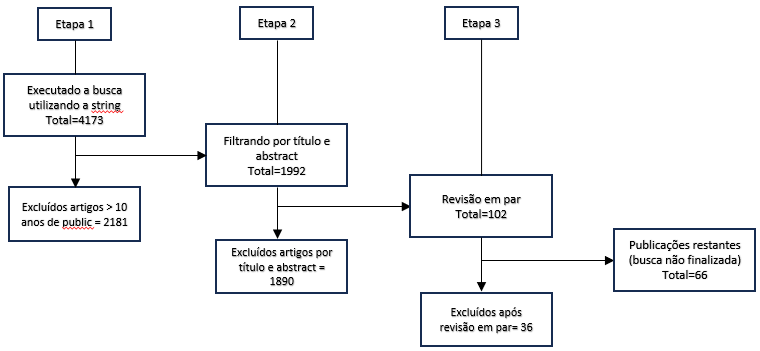
\includegraphics[width=1\textwidth]{img/rslteste.png}
\caption{Procedimento de seleção de estudos do teste.}
\label{fig:rsltest}
\end{figure}

Apesar do último filtro de artigos não ter sido realizado durante a fase de teste, entendeu-se que para o proposito de testes, esse esforço era o suficiente. As experiências obtidas através desse teste conseguiu esclarecer os principais pontos elencados no início desse seção além de mais algumas respostas:

 \begin{enumerate}
     \item Foi possível entender um pouco sobre a forma e sutiliza da execução das pesquisas entre diferentes repositórios de busca;
     \item Ter uma noção do sobre a quantidade de documentos que precisarão ser filtrados durante o processo de seleção dos estudos primários;
     \item Ter também uma ideia doo tempo necessário para realizar esse seleção;
     \item Foi possível também perceber que a string de busca muito genéria traz um resultado com muitos documentos, e que esse string precisaria ser refinada;
     \item Foi possível refinar e desenhar um melhor processo para a execução da pesquisa;
 \end{enumerate}
% ---------------------------------------------------------
% Plano de Trabalho e Cronograma

% ---
% Cronograma de Trabalho
% ---
\chapter{PLANO DE TRABALHO E CRONOGRAMA}
\label{cap:plano_cronograma}
% ---
Nesse capítulo, é apresentado um macro cronograma das próximas etapas de execução desse trabalho.

\textbf{Macro cronograma de atividades}:
\begin{itemize}
    \item \textbf{2023 - AGO:} Execução da Revisão sistemática de literatura - Repositório IEEE;
    \item \textbf{2023 - SET:} Apresentação da qualificação;
    \item \textbf{2023 - OUT:} Execução da Revisão sistemática de literatura - Repositórios ACM e Science Direct;
    \item \textbf{2023 - NOV:} Execução da Revisão sistemática de literatura - Repositórios Springer Link, Scopus e Citeseer Library;
    \item \textbf{2023 - DEZ:} Execução da Revisão sistemática de literatura - Repositórios SciElo e ArXvid;
    \item \textbf{2024 - JAN:} Criação do Artigo e Submissão de trabalho científico;
    \item \textbf{2024 - FEV:} Checklist;
    \item \textbf{2024 - MAR:} Finalização do texto da dissertação;
    \item \textbf{2024 - ABR} Apresentação da dissertação;
\end{itemize}

% ---------------------------------------------------------

% ------------------------------------------------------------------------
% FIM ELEMENTOS TEXTUAIS
% ------------------------------------------------------------------------
% ------------------------------------------------------------------------
% ------------------------------------------------------------------------

% ------------------------------------------------------------------------
% ------------------------------------------------------------------------
% ------------------------------------------------------------------------
% ELEMENTOS PÓS-TEXTUAIS
% ------------------------------------------------------------------------
\postextual

% ------------------------------------------------------------------------
% REFERÊNCIAS BIBLIOGRÁFICAS 
\bibliography{1000_bibliograf}

% ----------------------------------------------------------
% GLOSSÁRIO
% Consulte o manual da classe abntex2 para orientações sobre o glossário.
%\glossary

% ----------------------------------------------------------
% APÊNDICES
% Texto ou documento elaborado pelo autor, 
% a fim de complementar sua argumentação, sem prejuízo da 
% unidade nuclear do trabalho
%
% ----------------------------------------------------------
% Apêndices
% ----------------------------------------------------------

% ---
% Inicia os apêndices
% ---
\begin{apendicesenv}

% Imprime uma página indicando o início dos apêndices
\partapendices

% ----------------------------------------------------------
\chapter{Quisque libero justo}
% ----------------------------------------------------------

\lipsum[50]

% ----------------------------------------------------------
\chapter{Nullam elementum urna vel imperdiet sodales elit ipsum pharetra ligula
ac pretium ante justo a nulla curabitur tristique arcu eu metus}
% ----------------------------------------------------------
\lipsum[55-57]

\end{apendicesenv}

% ----------------------------------------------------------
% ANEXOS
% Texto ou documento não elaborado pelo autor, que serve de 
% fundamentação, comprovação e ilustração
%
% ----------------------------------------------------------
% Anexos
% ----------------------------------------------------------

% ---
% Inicia os anexos
% ---
\begin{anexosenv}

% Imprime uma página indicando o início dos anexos
\partanexos

% ---
\chapter{Morbi ultrices rutrum lorem.}
% ---
\lipsum[30]

% ---
\chapter{Cras non urna sed feugiat cum sociis natoque penatibus et magnis dis
parturient montes nascetur ridiculus mus}
% ---

\lipsum[31]

% ---
\chapter{Fusce facilisis lacinia dui}
% ---

\lipsum[32]

\end{anexosenv}

%---------------------------------------------------------------------
% INDICE REMISSIVO
\phantompart
\printindex
% ------------------------------------------------------------------------
% FIM ELEMENTOS PÓS-TEXTUAIS
% ------------------------------------------------------------------------
% ------------------------------------------------------------------------
% ------------------------------------------------------------------------

\end{document}